\documentclass[journal, onecolumn, 12pt]{IEEEtran}

% ========================
% Packages
% ========================
\usepackage{cite}
\usepackage{amsmath,amssymb,amsfonts}
\usepackage{algorithmic}
\usepackage{graphicx}
\usepackage{textcomp}
\usepackage{xcolor}
\usepackage{booktabs}       % For nicer tables
\usepackage{multirow}       % For multi-row cells
\usepackage{listings}       % For code inclusion
\usepackage{geometry}
\usepackage[table]{xcolor}  % For cell coloring
\usepackage{placeins}       % For \FloatBarrier

% ========================
% Custom Pastel Colors
% ========================
\definecolor{mygreen}{rgb}{0.7, 1, 0.7}   % Light Green
\definecolor{myyellow}{rgb}{1, 1, 0.7}    % Light Yellow
\definecolor{myred}{rgb}{1, 0.7, 0.7}     % Light Red

% ========================
% Page Margins
% ========================
\geometry{letterpaper, top=1in, bottom=1in, left=1in, right=1in}

% ========================
% Code Listing Style
% ========================
\definecolor{codegreen}{rgb}{0,0.6,0}
\definecolor{codegray}{rgb}{0.5,0.5,0.5}
\definecolor{codepurple}{rgb}{0.58,0,0.82}
\definecolor{backcolour}{rgb}{0.95,0.95,0.92}

\lstdefinestyle{mystyle}{
    backgroundcolor=\color{backcolour},   
    commentstyle=\color{codegreen},
    keywordstyle=\color{magenta},
    numberstyle=\tiny\color{codegray},
    stringstyle=\color{codepurple},
    basicstyle=\ttfamily\footnotesize,
    breakatwhitespace=false,         
    breaklines=true,                 
    captionpos=b,                    
    keepspaces=true,                 
    numbers=left,                    
    numbersep=5pt,                  
    showspaces=false,                
    showstringspaces=false,
    showtabs=false,                  
    tabsize=2
}

\lstset{style=mystyle}

% ========================
% Title Information
% ========================
\title{ECE275: Homework \#2}
\author{John R. Minnick\\
ECE 275: Electricity Market, Policy, and Modeling \\
Department of Electrical and Computer Engineering\\
March, 2026\\
\thanks{\textbf{Disclaimer:} Generative AI was used for the creation of the structure of this document as well as in some of the implementation of the underlying code used for modeling. However, all written content and opinions on matters herein are solely those of the author.}
}

\begin{document}

\maketitle

% ========================
% Problem 1: Least-Cost Dispatch with DC Load Flow
% ========================
\section{Least-Cost Dispatch with Transmission Constraints}

\subsection{Problem Setup}
\textit{Consider a 3-node triangle network (A, B, C) with 200 MW demand at each node. 
Node C has 500 MW capacity at \$26/MWh; Node B has 250 MW capacity at \$22/MWh. 
Reactances: A-B = 6.0, B-C = 6.0, A-C = 4.8. 
Link A-B has a flow limit of 45 MW in each direction.}\\

Nodes A, B, and C form a triangle network, each carrying 200 MW of demand for a total of 600 MW. Two generators serve this load: a 250 MW plant at node B (\$22/MWh) and a 500 MW plant at node C (\$26/MWh). Node A has no local generation and must be supplied entirely through transmission. \par

The links have reactances $R_{AB} = R_{BC} = 6.0\ \Omega$ and $R_{AC} = 4.8\ \Omega$, forming a single independent voltage loop ($A \to B \to C \to A$). Power splits across parallel paths according to Kirchhoff's Laws \cite{stoft2002} (Ch.~5-1, p.~376). Because A-C has a lower reactance, it carries a larger share of any loop flow. The A-B link is constrained to 45 MW in each direction; all other links are unconstrained.

\FloatBarrier
\begin{figure}[h]
    \centering
    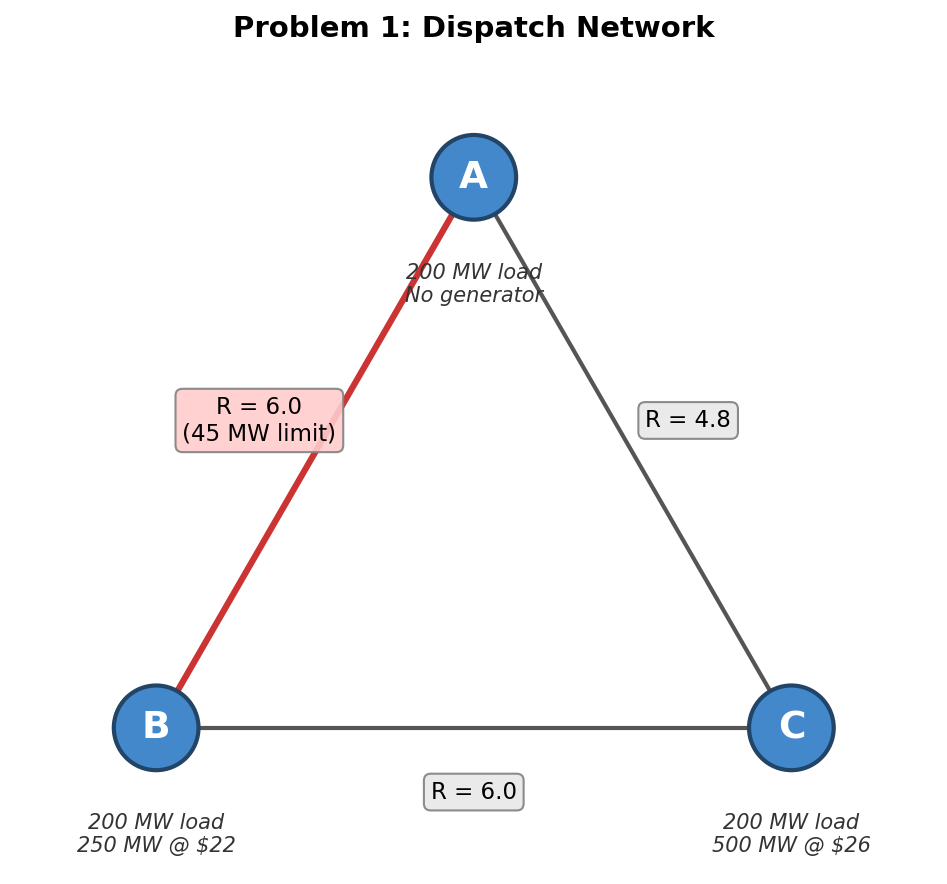
\includegraphics[width=0.55\textwidth]{hw2_network_p1.png}
    \caption{Three-node triangle network for Problem 1. Generators at B and C serve 200 MW demand at each node. The A-B link (red) has a 45 MW flow limit.}
    \label{fig:network_p1}
\end{figure}
\FloatBarrier

\subsection{Part A: LP Formulation and Constrained Dispatch}

We formulate a linear program with generation variables ($g_B$, $g_C$) and positive flow components ($t_{mn}$, $t_{nm}$) on each link. Net flow from $m$ to $n$ equals ($t_{mn} - t_{nm}$). This decomposition lets us express the 45 MW flow limit as simple upper bounds on the $t$ variables. The LP approach follows the competitive locational pricing framework described in \cite{stoft2002} (Ch.~5-3, pp.~392--394), which shows that only competitive locational prices minimize total production cost (Result~5-3.2).

The objective minimizes total cost: $\min\ 22g_B + 26g_C$. The constraints enforce power balance at each node (KCL) and zero net voltage drop around the loop (KVL):

\textbf{KCL (power balance at each node):}
\begin{align}
    \text{Node A:} \quad & (t_{BA} - t_{AB}) + (t_{CA} - t_{AC}) = 200 \label{eq:kcl_a}\\
    \text{Node B:} \quad & g_B + (t_{AB} - t_{BA}) + (t_{CB} - t_{BC}) = 200 \label{eq:kcl_b}\\
    \text{Node C:} \quad & g_C + (t_{AC} - t_{CA}) + (t_{BC} - t_{CB}) = 200 \label{eq:kcl_c}
\end{align}

\textbf{KVL (voltage loop):}
\begin{equation}
    6.0(t_{AB} - t_{BA}) + 6.0(t_{BC} - t_{CB}) - 4.8(t_{AC} - t_{CA}) = 0 \label{eq:kvl}
\end{equation}

\textbf{Bounds:}
\begin{equation}
    0 \leq g_B \leq 250, \quad 0 \leq g_C \leq 500, \quad 0 \leq t_{AB}, t_{BA} \leq 45
\end{equation}

Solving with HiGHS yields the dispatch in Table~\ref{tab:constrained}.

\begin{table}[h]
    \centering
    \caption{Constrained Dispatch Results (A-B limit = 45 MW)}
    \label{tab:constrained}
    \begin{tabular}{@{}lrr@{}}
    \toprule
    \textbf{Variable} & \textbf{Value} & \textbf{Unit} \\ \midrule
    Total Cost & \$14,936.00 & \\
    Gen B & 166.0 & MW \\
    Gen C & 434.0 & MW \\
    Flow B$\to$A (net) & 45.0 & MW \\
    Flow C$\to$B (net) & 79.0 & MW \\
    Flow C$\to$A (net) & 155.0 & MW \\
    \bottomrule
    \end{tabular}
\end{table}

The A-B link is binding at 45 MW (B to A). Power from C splits two ways: 155 MW goes directly to A, and 79 MW goes to B. Of the power arriving at B, some serves B's local 200 MW load, and the rest (45 MW) is forwarded to A. \par

Because A-B is congested, the optimizer cannot fully use the cheaper Gen B. In a pure merit-order dispatch, Gen B would run at its full 250 MW before turning to Gen C. Instead, the constraint holds Gen B to 166 MW, forcing Gen C up to 434 MW. This re-dispatch away from merit order is the direct cost of congestion.

\subsection{Part B: Locational Marginal Prices (LMPs)}
\textit{What is the marginal cost of meeting demand at each node?}\\

The dual variables on the KCL constraints (Equations~\ref{eq:kcl_a}--\ref{eq:kcl_c}) give the LMP at each node: the cost of serving one more MW of demand at that location \cite{stoft2002} (Ch.~5-3, Result~5-3.1, p.~392). These were verified by incrementing load 1 MW at each node and re-solving; the cost changes matched the duals exactly.

\begin{table}[h]
    \centering
    \caption{Locational Marginal Prices}
    \label{tab:lmps}
    \begin{tabular}{@{}lr@{}}
    \toprule
    \textbf{Node} & \textbf{LMP (\$/MWh)} \\ \midrule
    A & \cellcolor{myred} \$29.20 \\
    B & \cellcolor{mygreen} \$22.00 \\
    C & \cellcolor{myyellow} \$26.00 \\
    \bottomrule
    \end{tabular}
\end{table}

\textbf{Node B (\$22.00/MWh):} One more MW at B is met by raising Gen B by 1 MW. Gen B has spare capacity (166 of 250 MW dispatched) and no transmission constraint is affected, so the cost is simply its marginal cost. \par

\textbf{Node C (\$26.00/MWh):} Same logic. Gen C has spare capacity (434 of 500 MW), the extra demand and generation are co-located, and no new transmission is needed. \par

\textbf{Node A (\$29.20/MWh):} Node A's LMP exceeds both generators' marginal costs. This seems wrong at first. How can power cost more at A than at either place it is produced? \par

The answer is that A has no generator and the B-to-A link is full. An extra MW at A cannot be served by simply raising Gen B, because the 45 MW limit blocks it. Nor can Gen C just add 1 MW and send it to A directly, because the KVL equation ties all three link flows together: changing one flow forces changes on the others. \par

What happens instead is that the system raises Gen C and lowers Gen B in a ratio set by the network physics, routing the extra power to A through the unconstrained C-A path while keeping the loop flows balanced. The net cost of swapping cheap B generation (\$22) for expensive C generation (\$26), plus the loop flow adjustments, comes to \$29.20/MWh. Congestion makes power at A more expensive than at either source.

\subsection{Part C: Cost of Congestion}
\textit{How much money would be saved if there were no transmission constraints?}\\

Relaxing the A-B limit and re-solving gives the unconstrained optimum, shown in Table~\ref{tab:congestion_cost}.

\begin{table}[h]
    \centering
    \caption{Cost of Congestion}
    \label{tab:congestion_cost}
    \begin{tabular}{@{}lr@{}}
    \toprule
    \textbf{Scenario} & \textbf{Total Cost} \\ \midrule
    Constrained (45 MW limit) & \$14,936.00 \\
    Unconstrained (no limit) & \$14,600.00 \\
    \textbf{Cost of Congestion} & \cellcolor{myred} \textbf{\$336.00} \\
    \bottomrule
    \end{tabular}
\end{table}

Without the constraint, the optimizer runs Gen B at its full 250 MW before dispatching Gen C for the remaining 350 MW. Total cost drops to \$14,600, so the cost of congestion is \textbf{\$336}. \par

The constraint becomes non-binding at 75 MW. In the unconstrained dispatch, the natural B-to-A flow (set by the impedances and injection pattern) is exactly 75 MW. Any limit at or above that level has no effect on the solution. Figure~\ref{fig:sensitivity} illustrates this relationship.

\FloatBarrier
\begin{figure}[h]
    \centering
    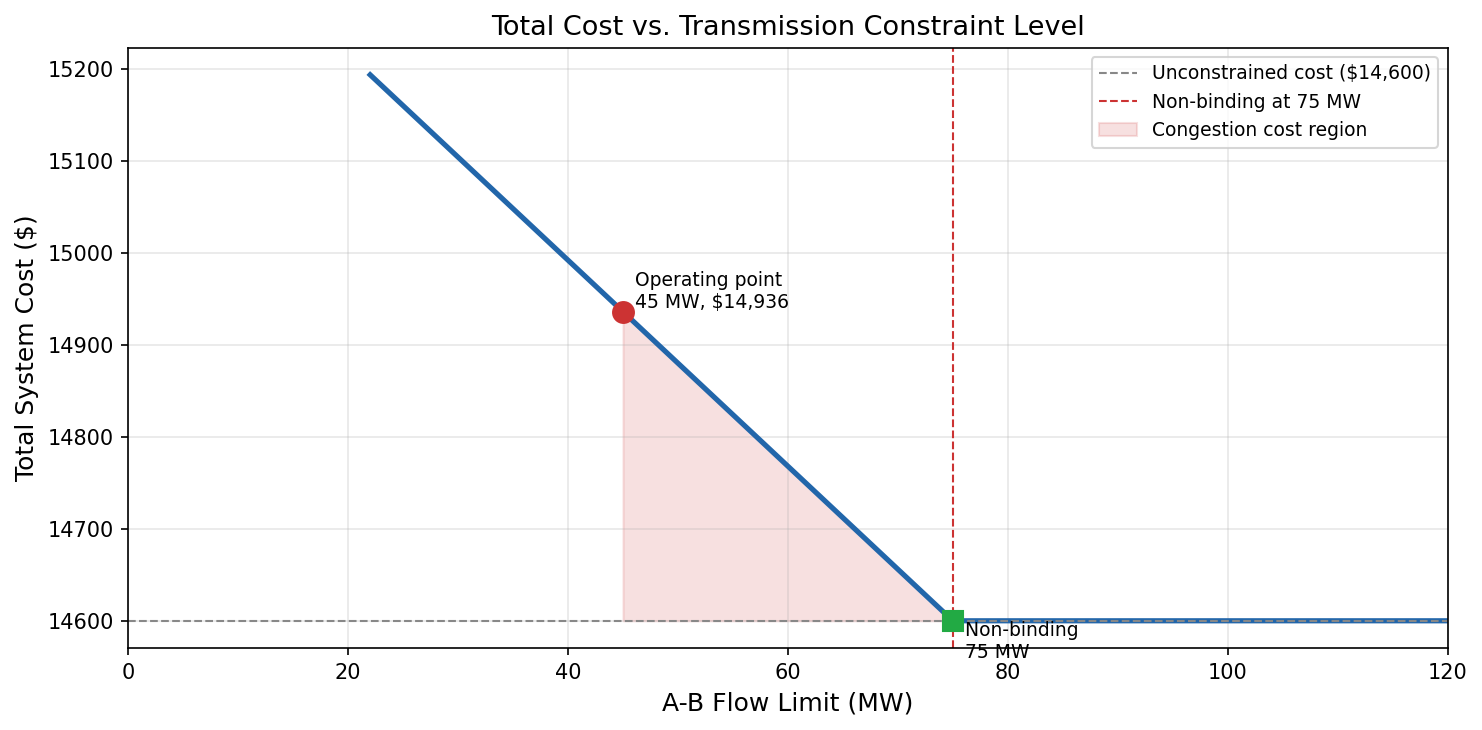
\includegraphics[width=0.85\textwidth]{hw2_sensitivity.png}
    \caption{Total system cost as a function of the A-B flow limit. At the current operating point (45 MW), congestion adds \$336 to the system cost. The constraint becomes non-binding at 75 MW, beyond which cost remains flat at \$14,600.}
    \label{fig:sensitivity}
\end{figure}
\FloatBarrier

\subsection{Part D: Congestion Surplus}
\textit{Calculate the ISO's ``congestion surplus'' and compare it to the cost of congestion.}\\

In an LMP market, the ISO charges consumers the local LMP for withdrawals and pays generators the local LMP for injections. When congestion creates price differences between nodes, the ISO collects more than it pays out. This net revenue is the ``congestion surplus.'' \par

\textbf{Consumer Payments:}
\begin{align*}
    \text{Consumers} &= \text{LMP}_A \times D_A + \text{LMP}_B \times D_B + \text{LMP}_C \times D_C \\
    &= \$29.20 \times 200 + \$22.00 \times 200 + \$26.00 \times 200 \\
    &= \$5{,}840 + \$4{,}400 + \$5{,}200 = \$15{,}440.00
\end{align*}

\textbf{Generator Revenue:}
\begin{align*}
    \text{Generators} &= \text{LMP}_B \times g_B + \text{LMP}_C \times g_C \\
    &= \$22.00 \times 166 + \$26.00 \times 434 \\
    &= \$3{,}652 + \$11{,}284 = \$14{,}936.00
\end{align*}

\textbf{Congestion Surplus:}
$$\text{Congestion Surplus} = \$15{,}440 - \$14{,}936 = \textbf{\$504.00}$$

The congestion surplus (\$504) is \textbf{not equal} to the cost of congestion (\$336). They measure different things. The cost of congestion is the extra production cost from re-dispatching away from merit order. The congestion surplus is the revenue the ISO collects from price spreads between nodes. Stoft addresses this directly in \cite{stoft2002} (Ch.~5-5, Fallacy~5-5.1, p.~406): the fact that congestion rent exceeds redispatch cost is not a market failure but a natural consequence of locational pricing. The surplus exceeds the production cost increase because it reflects the full price differential applied to all demand, not just the incremental fuel cost. In practice, this surplus is allocated to Financial Transmission Rights (FTR) holders \cite{stoft2002} (Ch.~5-9, pp.~433--440) or used to fund transmission upgrades.

\FloatBarrier
\begin{figure}[h]
    \centering
    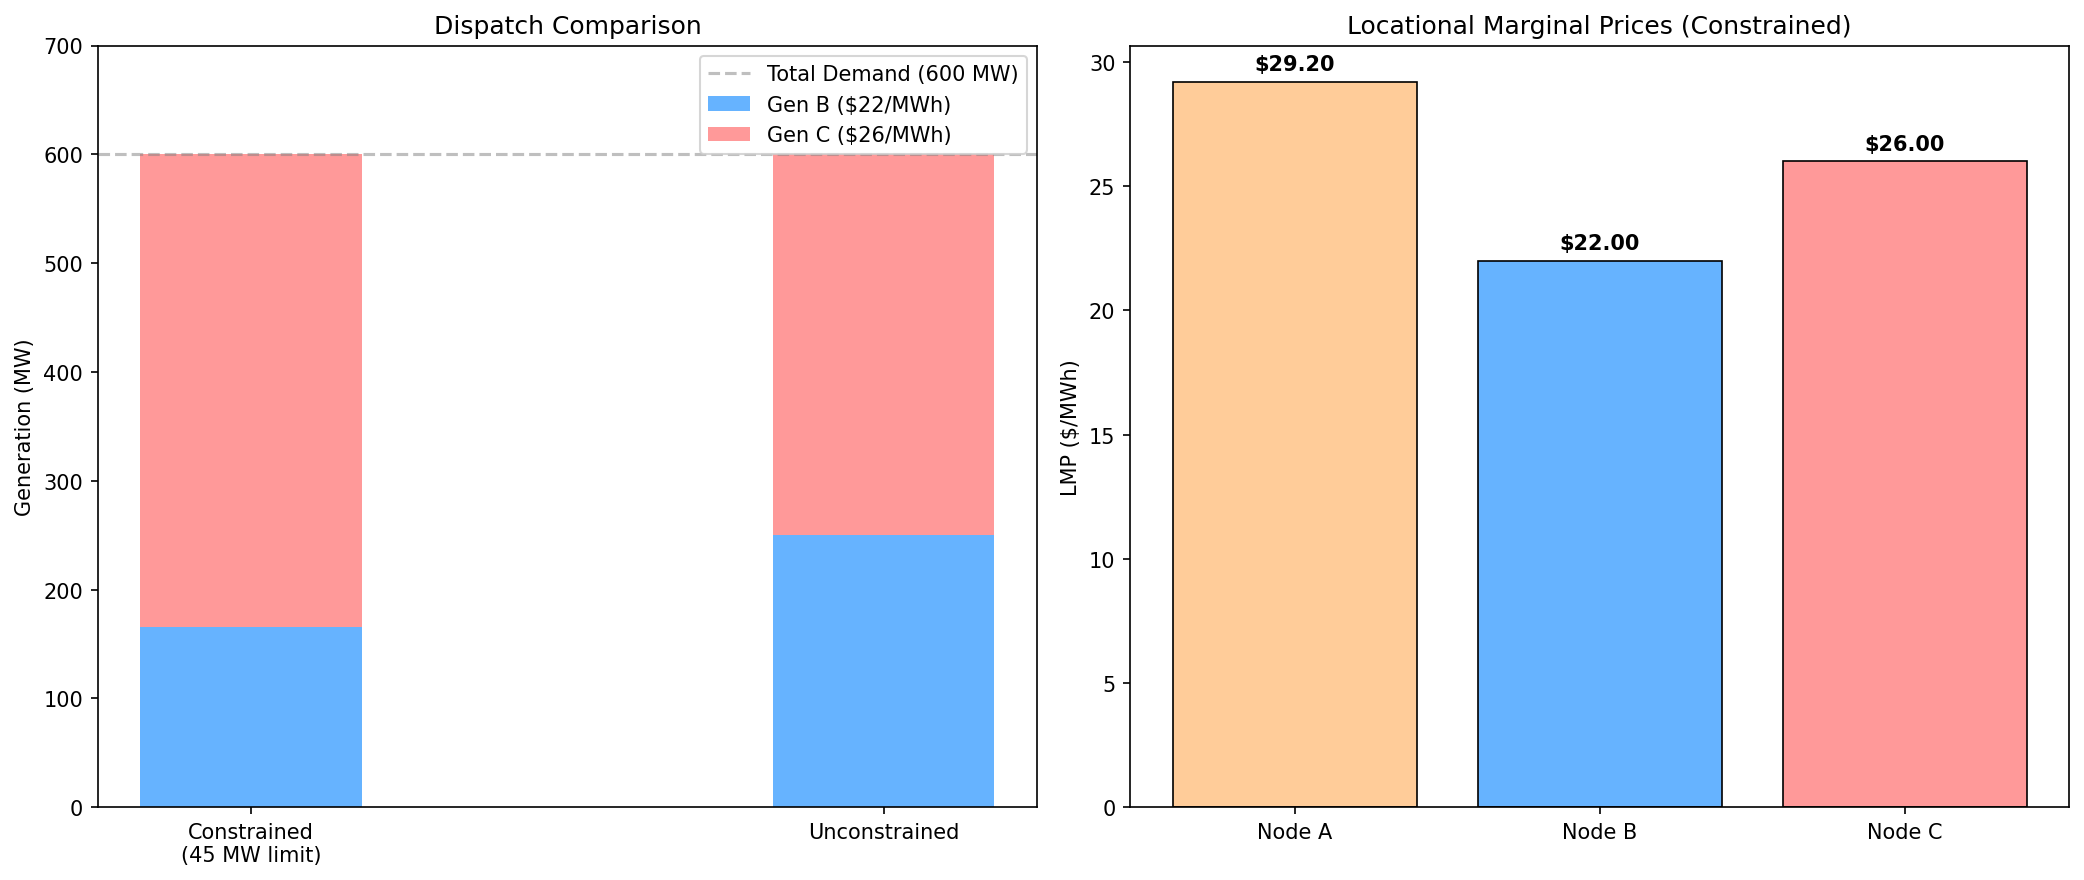
\includegraphics[width=0.85\textwidth]{hw2_dispatch.png}
    \caption{Left: Generation dispatch with and without the 45 MW constraint. The constraint forces Gen B from 250 MW down to 166 MW. Right: LMPs under congestion. Node A's price (\$29.20) exceeds both generators because it sits behind a congested link with no local supply.}
    \label{fig:hw2_dispatch}
\end{figure}
\FloatBarrier

\newpage

% ========================
% Problem 2: PTDF Calculation
% ========================
\section{Power Transmission Distribution Factors (PTDFs)}

\subsection{Problem Setup}
\textit{Same 3-node triangle network. Reactances: A-B = 1.7, B-C = 1.7, A-C = 1.4. Hub node is A. Calculate PTDFs for injections at various nodes.}\\

$\text{PTDF}_{m,jk}$ gives the flow induced on line $j \to k$ by a 1 MW injection at node $m$ with a matching withdrawal at the hub \cite{stoft2002} (Ch.~5-4, Result~5-4.1, p.~397). Because the DC load flow is linear, these factors scale proportionally: a 10 MW injection produces ten times the flow of a 1 MW injection. \par

For this problem, the reactances differ from Problem 1: $R_{AB} = R_{BC} = 1.7\ \Omega$ and $R_{AC} = 1.4\ \Omega$. Node A is the hub.

\FloatBarrier
\begin{figure}[h]
    \centering
    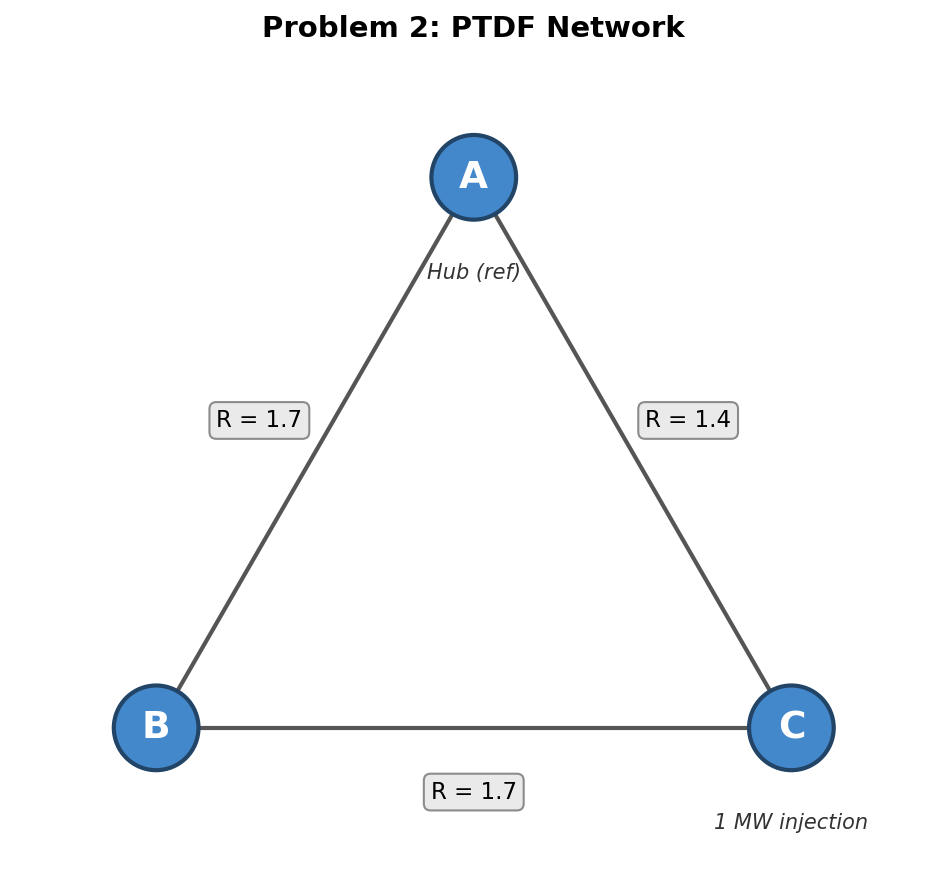
\includegraphics[width=0.55\textwidth]{hw2_network_p2.png}
    \caption{Three-node triangle network for Problem 2 (PTDF). Node A is the hub (reference). Reactances differ from Problem 1.}
    \label{fig:network_p2}
\end{figure}
\FloatBarrier

\subsection{Methodology}

\begin{enumerate}
    \item Compute line susceptances: $b_{mn} = 1/R_{mn}$. Lower reactance means higher susceptance and more flow.
    \item Build the full nodal susceptance matrix $\mathbf{B}$ (3$\times$3).
    \item Remove the hub node (A) to get $\mathbf{B}_{\text{red}}$ (2$\times$2), since the hub angle is fixed at zero.
    \item Invert: $\mathbf{X} = \mathbf{B}_{\text{red}}^{-1}$.
    \item Each PTDF is: $\text{PTDF}_{m, j \to k} = b_{jk} \cdot (X_{mj} - X_{mk})$, with $X_{A,*} = 0$.
\end{enumerate}

\subsection{Susceptance Matrix and Inversion}

$$b_{AB} = b_{BC} = \frac{1}{1.7} \approx 0.5882, \quad b_{AC} = \frac{1}{1.4} \approx 0.7143$$

$$\mathbf{B}_{\text{red}} = \begin{pmatrix} 1.1765 & -0.5882 \\ -0.5882 & 1.3025 \end{pmatrix}, \quad \mathbf{X} = \mathbf{B}_{\text{red}}^{-1} = \begin{pmatrix} 1.0979 & 0.4958 \\ 0.4958 & 0.9917 \end{pmatrix}$$

Rows and columns of $\mathbf{X}$ correspond to B (index 0) and C (index 1). Hub node A entries are zero.

\subsection{PTDF Results}

\begin{table}[h]
    \centering
    \caption{PTDF Calculations (Hub = A)}
    \label{tab:ptdfs}
    \begin{tabular}{@{}lcl@{}}
    \toprule
    \textbf{PTDF} & \textbf{Value} & \textbf{Calculation} \\ \midrule
    $\text{PTDF}_{C,AB}$ & $-0.2917$ & $b_{AB}(X_{CA} - X_{CB}) = 0.5882(0 - 0.4958)$ \\
    $\text{PTDF}_{C,BA}$ & $+0.2917$ & $b_{BA}(X_{CB} - X_{CA}) = 0.5882(0.4958 - 0)$ \\
    $\text{PTDF}_{C,AC}$ & $-0.7083$ & $b_{AC}(X_{CA} - X_{CC}) = 0.7143(0 - 0.9917)$ \\
    $\text{PTDF}_{C,BC}$ & $-0.2917$ & $b_{BC}(X_{CB} - X_{CC}) = 0.5882(0.4958 - 0.9917)$ \\
    $\text{PTDF}_{B,AC}$ & $-0.3542$ & $b_{AC}(X_{BA} - X_{BC}) = 0.7143(0 - 0.4958)$ \\
    $\text{PTDF}_{A,AC}$ & $0.0000$ & $b_{AC}(X_{AA} - X_{AC}) = 0.7143(0 - 0)$ \\
    \bottomrule
    \end{tabular}
\end{table}

\subsection{Interpretation}

For a 1 MW injection at C with withdrawal at hub A, the power splits two ways. About 70.8\% flows directly from C to A ($|\text{PTDF}_{C,AC}| = 0.7083$), and the remaining 29.2\% takes the path C $\to$ B $\to$ A ($|\text{PTDF}_{C,BC}| = |\text{PTDF}_{C,AB}| = 0.2917$). The A-C link attracts the larger share because it has the lower reactance (1.4 vs 1.7). These two fractions sum to 1.0, confirming all power leaving C is accounted for. \par

$\text{PTDF}_{C,BA} = -\text{PTDF}_{C,AB}$: reversing a line's direction negates the PTDF, as expected. The physical flow is unchanged; only the sign convention differs. \par

For a 1 MW injection at B with withdrawal at A, $\text{PTDF}_{B,AC} = -0.3542$ says that 35.4\% of the power appears on the A-C link, flowing from C toward A. At first glance, all power should flow straight from B to A, but the KVL constraint forces some flow to circulate through the loop, inducing flow on all three lines. \par

$\text{PTDF}_{A,AC} = 0$: injecting and withdrawing at the same node (the hub) means zero net injection, so no flows are induced on any line.

\newpage

% ========================
% Appendix: Python Code
% ========================
\section{Appendix: Python Code}
\begin{lstlisting}[language=Python, caption=DC Load Flow and PTDF Calculation Code]
"""
ECE275 Homework 2: Linearized DC Load Flow
Solves: (1) Least-Cost Dispatch with Transmission Constraints
        (2) PTDF Calculation
"""
import numpy as np
from scipy.optimize import linprog
import matplotlib.pyplot as plt

def solve_dispatch():
    """Problem 1: LP-based dispatch with KCL/KVL constraints."""
    # Demand (MW) and generator data
    D_A, D_B, D_C = 200.0, 200.0, 200.0
    Cap_B, MC_B = 250.0, 22.0
    Cap_C, MC_C = 500.0, 26.0
    R_AB, R_BC, R_AC = 6.0, 6.0, 4.8
    F_AB_max = 45.0

    # Decision vars: [g_B, g_C, t_AB, t_BA, t_BC, t_CB, t_AC, t_CA]
    c = np.array([MC_B, MC_C, 0, 0, 0, 0, 0, 0])

    A_eq = np.array([
        [0, 0, -1, 1, 0, 0, -1, 1],        # KCL Node A
        [1, 0,  1,-1,-1, 1,  0, 0],         # KCL Node B
        [0, 1,  0, 0, 1,-1,  1,-1],         # KCL Node C
        [0, 0, R_AB,-R_AB, R_BC,-R_BC, -R_AC, R_AC],  # KVL
    ], dtype=float)
    b_eq = np.array([D_A, D_B, D_C, 0.0])

    big_M = 10000.0
    bounds_con = [(0,Cap_B),(0,Cap_C),(0,F_AB_max),(0,F_AB_max),
                  (0,big_M),(0,big_M),(0,big_M),(0,big_M)]
    bounds_uncon = [(0,Cap_B),(0,Cap_C),(0,big_M),(0,big_M),
                    (0,big_M),(0,big_M),(0,big_M),(0,big_M)]

    res_con = linprog(c, A_eq=A_eq, b_eq=b_eq, bounds=bounds_con, method='highs')
    res_uncon = linprog(c, A_eq=A_eq, b_eq=b_eq, bounds=bounds_uncon, method='highs')

    # LMPs from dual variables
    duals = res_con.eqlin.marginals
    LMP_A, LMP_B, LMP_C = duals[0], duals[1], duals[2]

    # Congestion surplus
    x = res_con.x
    consumer_pay = LMP_A*D_A + LMP_B*D_B + LMP_C*D_C
    gen_rev = LMP_B*x[0] + LMP_C*x[1]
    surplus = consumer_pay - gen_rev

    print(f"Constrained: Cost=${res_con.fun:,.2f}, B={x[0]:.0f}MW, C={x[1]:.0f}MW")
    print(f"Unconstrained: Cost=${res_uncon.fun:,.2f}")
    print(f"LMPs: A=${LMP_A:.2f}, B=${LMP_B:.2f}, C=${LMP_C:.2f}")
    print(f"Congestion cost: ${res_con.fun - res_uncon.fun:,.2f}")
    print(f"Congestion surplus: ${surplus:,.2f}")

def solve_ptdf():
    """Problem 2: PTDF via susceptance matrix inversion."""
    b_AB = 1/1.7; b_BC = 1/1.7; b_AC = 1/1.4
    B_red = np.array([[b_AB+b_BC, -b_BC], [-b_BC, b_BC+b_AC]])
    X = np.linalg.inv(B_red)  # Rows/cols: B=0, C=1; A=hub (all zeros)

    def ptdf(m, j, k):
        idx = {'B':0, 'C':1}
        b = {'AB':b_AB,'BA':b_AB,'BC':b_BC,'CB':b_BC,'AC':b_AC,'CA':b_AC}
        X_mj = X[idx[m], idx[j]] if m!='A' and j!='A' else 0
        X_mk = X[idx[m], idx[k]] if m!='A' and k!='A' else 0
        return b[j+k] * (X_mj - X_mk)

    for name, args in [('C,AB',('C','A','B')), ('C,BA',('C','B','A')),
                        ('C,AC',('C','A','C')), ('C,BC',('C','B','C')),
                        ('B,AC',('B','A','C')), ('A,AC',('A','A','C'))]:
        print(f"PTDF_{{{name}}} = {ptdf(*args):.6f}")

if __name__ == "__main__":
    solve_dispatch()
    solve_ptdf()
\end{lstlisting}

\bibliographystyle{IEEEtran}
\bibliography{references}

\end{document}
